\documentclass[]{article}
\usepackage{lmodern}
\usepackage{amssymb,amsmath}
\usepackage{ifxetex,ifluatex}
\usepackage{fixltx2e} % provides \textsubscript
\ifnum 0\ifxetex 1\fi\ifluatex 1\fi=0 % if pdftex
  \usepackage[T1]{fontenc}
  \usepackage[utf8]{inputenc}
\else % if luatex or xelatex
  \ifxetex
    \usepackage{mathspec}
  \else
    \usepackage{fontspec}
  \fi
  \defaultfontfeatures{Ligatures=TeX,Scale=MatchLowercase}
\fi
% use upquote if available, for straight quotes in verbatim environments
\IfFileExists{upquote.sty}{\usepackage{upquote}}{}
% use microtype if available
\IfFileExists{microtype.sty}{%
\usepackage{microtype}
\UseMicrotypeSet[protrusion]{basicmath} % disable protrusion for tt fonts
}{}
\usepackage{hyperref}
\hypersetup{unicode=true,
            pdfborder={0 0 0},
            breaklinks=true}
\urlstyle{same}  % don't use monospace font for urls
\usepackage{graphicx,grffile}
\makeatletter
\def\maxwidth{\ifdim\Gin@nat@width>\linewidth\linewidth\else\Gin@nat@width\fi}
\def\maxheight{\ifdim\Gin@nat@height>\textheight\textheight\else\Gin@nat@height\fi}
\makeatother
% Scale images if necessary, so that they will not overflow the page
% margins by default, and it is still possible to overwrite the defaults
% using explicit options in \includegraphics[width = 7cm][width, height, ...]{}
\setkeys{Gin}{width=\maxwidth,height=\maxheight,keepaspectratio}
\IfFileExists{parskip.sty}{%
\usepackage{parskip}
}{% else
\setlength{\parindent}{0pt}
\setlength{\parskip}{6pt plus 2pt minus 1pt}
}
\setlength{\emergencystretch}{3em}  % prevent overfull lines
\providecommand{\tightlist}{%
  \setlength{\itemsep}{0pt}\setlength{\parskip}{0pt}}
\setcounter{secnumdepth}{0}
% Redefines (sub)paragraphs to behave more like sections
\ifx\paragraph\undefined\else
\let\oldparagraph\paragraph
\renewcommand{\paragraph}[1]{\oldparagraph{#1}\mbox{}}
\fi
\ifx\subparagraph\undefined\else
\let\oldsubparagraph\subparagraph
\renewcommand{\subparagraph}[1]{\oldsubparagraph{#1}\mbox{}}
\fi

\date{}

\begin{document}

\subsection{Title}\label{title}

Electrically actuated phase-change pixels for transmissive and
reflective spatial light modulators in the near and mid infrared

\subsection{Authors}\label{authors}

\begin{itemize}
\tightlist
\item
  JOSHUA HENDRICKSON
\item
  HAIBO LIANG
\item
  RICHARD SOREF
\item
  JIANWEI MU
\end{itemize}

\subsection{Abstract}\label{abstract}

An electrically actuated layer of phase-change material (PCM) was
employed to build the transmissive and reflective spatial light
modulators, the PCM was sandwiched between N-droped Si or indium tin
oxide layers.\\
Work at 1.55 (to 2.10) \(\mu m\), that is, near- and mid- infred
region.\\
Focus on modulating and switching free-space light.

\paragraph{Conclusion}\label{conclusion}

1.55 $\mu m$ wavelength where 0.7 dB IL and 27 dB C(R) are found in
reflective SLMs as compared to 4.5 dB IL and 32 dB C(T) in transmissive
SLMs. For both S and P polariza- tion the simulated performance was
relatively insensitive to angle variation in the 0° to 25° range

\paragraph{SIMULATIONS OF INDIVIDUAL TRANSMISSIVE SLM
PIXELS}\label{simulations-of-individual-transmissive-slm-pixels}

N-doped Si's donor concentration: \(1 \times 10^{19} \,cm^{-3}\)\\
Corresponding refractive index of Si: \(3.4807 + 0.0015i\) at
\(1.55\,\mu m\)\\
GST layer index: \(4.60 + 0.12i\) (amorphous), \(6.98 + 1.84i\)
(crystalline)\\
Thickness of GST layer: 100 to 500 nm\\
Thickness of doped semiconductor layer: 200 or 500 nm\\
\newpage
Structure of device:\\
\centerline{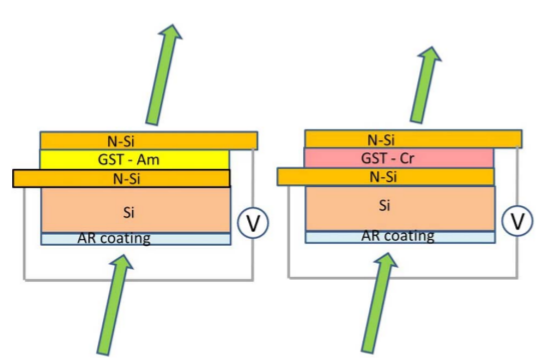
\includegraphics[width = 9cm]{image/002_01.png}}\\
Performance with different parameters:\\
\centerline{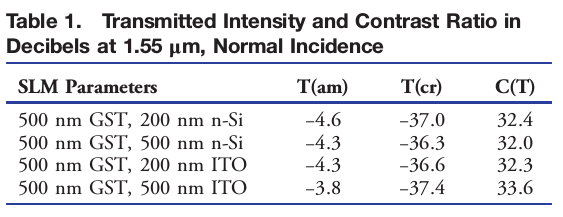
\includegraphics[width = 9cm]{image/002_02.png}}

\paragraph{SIMULATIONS OF INDIVIDUAL REFLECTIVE SLM
PIXELS}\label{simulations-of-individual-reflective-slm-pixels}

N-doped Si's donor concentration: \(1 \times 10^{19} \,cm^{-3}\)\\
Performance at optimal parameter:\\
\centerline{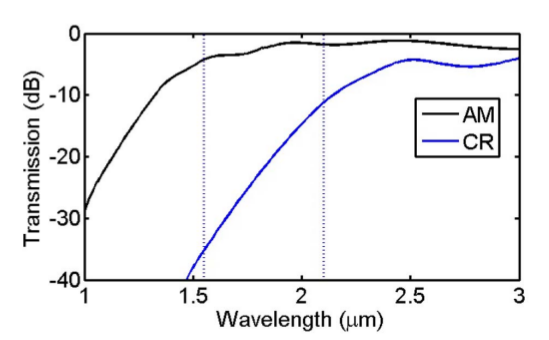
\includegraphics[width = 9cm]{image/002_03.png}}\\
\newpage
Structure:\\
\centerline{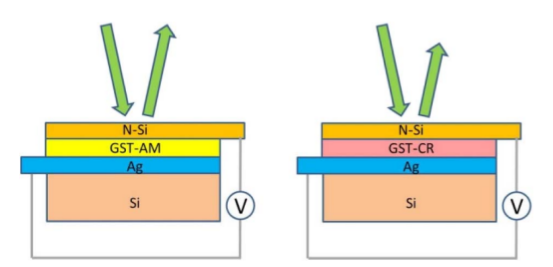
\includegraphics[width = 9cm]{image/002_04.png}}

\subsection{Highlight}\label{highlight}

\textbf{Electrical control} means that the PCM is sandwiched between two
transparent conductors with voltage applied across the conductors. An
applied field or current of suitable duration and strength then induces
the desired phase change. Advantageously, the PCM film is
\textbf{stable}, or \textbf{self-holding}, in either phase. External
electric power is utilized only during the brief time of phase
transition. The optical properties of the two phases differ rather
dramatically, and this optical difference has a variety of important
applications.

An \emph{antireflection (AR)} layer is useful in the transmissive SLM,
while in the reflective SLM a \emph{metallic mirror} layer replaces one
of the transparent conducting layers.

In the present work, we assume that the PCM layer is divided into a
two-dimensional (2D) N × M array of small pixel areas that are
electrically addressed as individuals. Addressing would be done by
structuring both electrical layers that contact the PCM. The front-plate
contact is divided into electrically separate \(X_i\) stripes, while the
rear-plate contact has orthogonal \(Y_j\) stripes, where i = 1\ldots{}N
and j = 1\ldots{}M, thereby providing \(X_i - Y_j\) addressing of
individual pixels in the PCM layer.

\paragraph{Performance at different incidence
angles}\label{performance-at-different-incidence-angles}

Calculated reflectivity as a function of incidence angle for both S and
P polarization in a device optimized at $\lambda$ < 1.55 $\mu m$.\\
\centerline{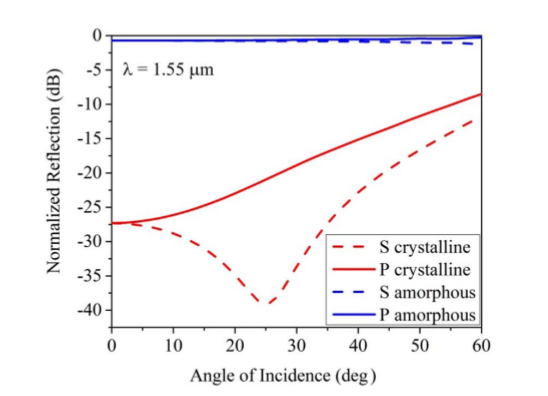
\includegraphics[width = 9cm]{image/002_05.png}}\\
Transmitted Am and Cr intensity versus angle of incidence for a 500 nm
GST film thickness at $\lambda$ < 1.55 $\mu m$ using 200 nm N-doped Si contacts.\\
\centerline{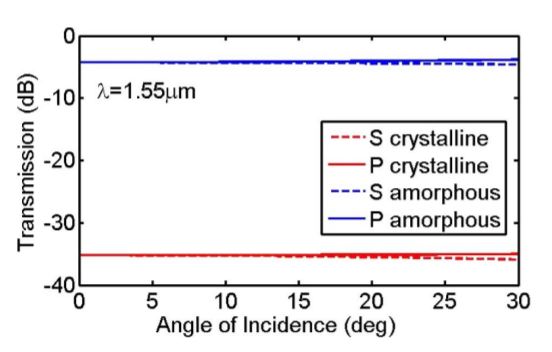
\includegraphics[width = 9cm]{image/002_09.png}}

\newpage
\paragraph{Real and imaginary indexes versus
wavelength}\label{real-and-imaginary-indexes-versus-wavelength}

N-doped Si:\\
\centerline{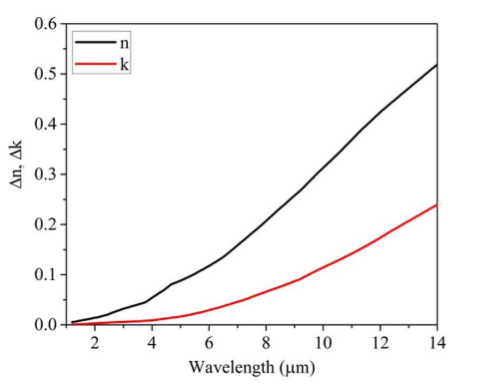
\includegraphics[width = 9cm]{image/002_06.png}}\\
GST:\\
\centerline{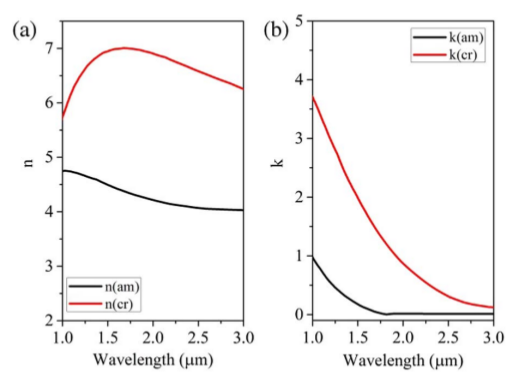
\includegraphics[width = 9cm]{image/002_07.png}}

\paragraph{Performance of transmissive
SLM}\label{performance-of-transmissive-slm}

Transmitted Am and Cr intensity versus GST film thickness at $\lambda$ < 1.55 $\mu m$
using 200 nm N-doped Si contacts.\\
\centerline{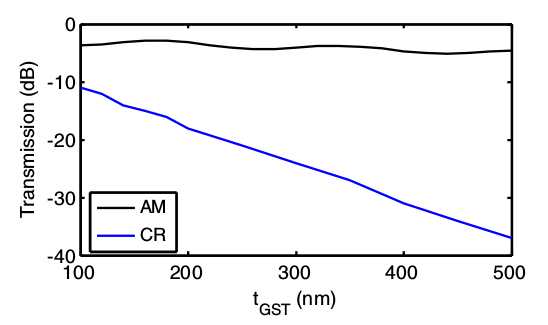
\includegraphics[width = 9cm]{image/002_08.png}}

\paragraph{Performance of reflective
SLM}\label{performance-of-reflective-slm}

Calculated reflectance as a function of wavelength for an EO device
optimized at $\lambda$ < 1.55 $\mu m$.\\
\centerline{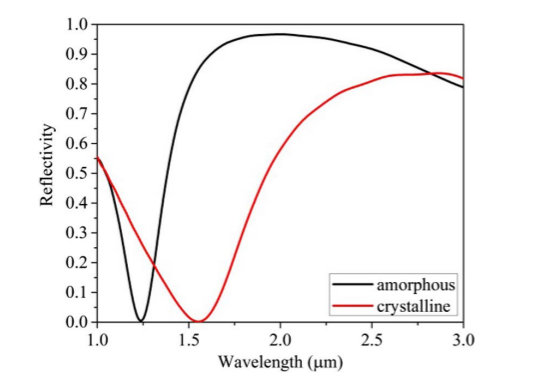
\includegraphics[width = 9cm]{image/002_10.png}}\\
Calculated reflectance as a function of wavelength for an EO device
optimized at $\lambda$ < 2.10 $\mu m$.\\
\centerline{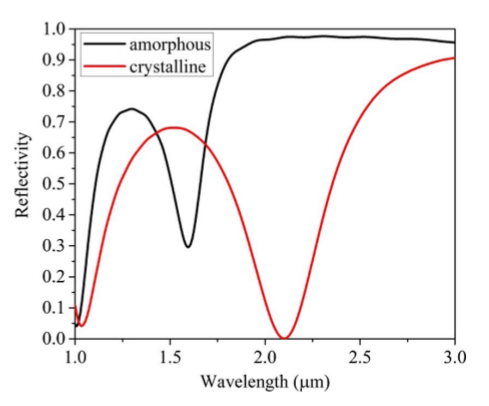
\includegraphics[width = 9cm]{image/002_11.png}}

\subsection{Related work}\label{related-work}

\paragraph{Issues}\label{issues}

\textbf{Challenge:} Implement a practical and effective technique for
electrical addressing and temporal multiplexing of the N × M array of
pixels in the PCM SLM.\\
\textbf{Solution:} We are proposing that the \textbf{LC addressing
structures} should be adapted and adopted in the PCM cases of
transmissive and reflective SLMs. Commercial devices are available with
logic supplies of \textless{}3.3 V and \textgreater{}12 V for driving
pixels. In the present case, the set and reset pulse amplitudes are
about 2 and 5 V, respectively, and the known circuitry can readily
provide that.

\textbf{Speed:} For 500 nm thick GST the \textbf{reset} pulse duration
is around \textbf{100 ns} and the \textbf{set} pulse duration is around
\textbf{1.5 ns}, with further reduction in GST thickness leading to
faster reset/set times.

\textbf{Gray scale enhancement:} Binary operation is not always
sufficient, and a scheme toextend our device performance from binary to
gray scale would help to increase the potential application space. We
speculate that moderate sized ``macro pixels,'' each composed of
\textbf{multiple individual black/white pixels}, could be used for
gray-scale production. Furthermore, gray-scale operation may also be
obtainable through the \textbf{stacking of multiple layers of PCMs
separated} by additional conducting layers within a given pixel. Here,
each independent phase change layer could be switched, allowing for
multiple (\textgreater{}2) transmission (reflection) value states for a
given pixel.

\textbf{Upper limit thickness:} Finally, we note that there is in
practice an upper limit on the PCM film thickness t which is determined
by the maximum electric power that is acceptable for addressing a given
pixel (the \(I^2 R\) Joule heating during reset is proportional to t).
With this in mind, we have taken \textbf{t = 500 nm as the upper limit}.

\paragraph{References}\label{references}

\begin{itemize}
\tightlist
\item
  Proposal of a small self-holding 2 × 2 optical switch using
  phase-change material
\item
  Electro-optical switching at 1550 nm using a two-state GeSe
  phase-change layer
\item
  Electro-optical 1 × 2, 1 × N, and N × N fiber optic and free-space
  switching over 1.55 to 3.0 \(\mu m\) using a
  \(\mathrm{Ge-Ge_2 Sb_2 Te_5 -Ge}\) prism structure
\item
  Simulations of silicon-on-insulator channel waveguide electrooptical 2
  × 2 switches and 1 × 1 modulators using a \(\mathrm{Ge_2 Sb_2 Te_5}\)
  self-holding layer
\item
  Electro-optic phase-change 2 × 2 switching using three- and
  four-waveguide directional couplers
\item
  Waveguide-size hybrid \(\mathrm{Si-VO_2}\) waveguide electroabsorption
  optical switches and photodetectors
\end{itemize}

\end{document}
